\chapter{Conceptos teóricos}

En este capítulo se describen (brevemente) todos los conceptos necesarios para entender el trabajo. No se trata de copiar el contenido de los libros de texto, si no de hacer un resumen de los conceptos necesarios para facilitar la lectura del documento al lector. Se entiende que el lector de un TFG tiene que tener unos conocimientos mínimos sobre el tema.

\section{¿Qué es la domótica?}

Desde el punto de vista etimológico, el término “domótica” proviene de la unión de las palabras \textit{“domus”}, que en latín significa casa, con la palabra griega \textit{“tica”}, cuya interpretación más acertada es “que trabaja por sí solo”. Por tanto, la palabra domótica podría traducirse como “la casa que trabaja de manera autónoma”. Fue acuñada a finales de los años 60 en Francia (\textit{“domotique”}) con la finalidad de crear nuevas palabras en su idioma para las tecnologías emergentes, en lugar de utilizar préstamos lingüísticos o anglicismos. Pero no fue hasta 1988 cuando apareció por primera vez recogida en un diccionario (“Enciclopedia Larousse”) con la siguiente definición \cite{Larousse:1988}: “Concepto de vivienda que integra automatismos en materia de seguridad, gestión de la energía, comunicaciones, etc”. \\\\
Posteriormente se han recogido descripciones más detalladas y acertadas del propio concepto domótica, como es el siguiente\cite{Quezada:2017}: “dícese de la parte de la tecnología (electrónica e informática) que integra el control y supervisión de los elementos existentes en un edificio de oficinas o de viviendas, garantizado por sistemas que realizan varias funciones y que pueden estar conectados entre sí a redes interiores y exteriores de comunicación. Gracias a ello se obtiene un notable ahorro de energía, una eficaz gestión técnica de la vivienda, una buena comunicación con el exterior y un alto nivel de seguridad”.\\\\
Entrando en una definición más formal y tangible del término, se materializa en una técnica física denominada “Sistema domótico”, que está formado por una serie de módulos y mecanismos conexionados entre sí por una red de comunicación a través de un bus de datos, lo que permite el intercambio de información a través de diferentes protocolos de comunicación. Incluso, se suele incluir algún tipo de interfaz que permita a una persona ser partícipe de la concurrencia de toda esta información.\\\\
Todo esto tendrá como fin la automatización de una vivienda, es decir, que varias de las actividades que hasta ahora estaban destinadas a ser realizadas por las personas que las habitaban, pasan a ser tarea del sistema domótico instalado en ella, reduciendo así la necesidad de vigilarlas y controlarlas de manera directa, y logrando adecuar las condiciones ambientales para ofrecer a los inquilinos las mayores prestaciones de confort y seguridad posibles.\\\\
A lo largo de este Trabajo de Fin de Máster se irán desgranando los diferentes procesos necesarios para que una vivienda convencional evolucione hacia el hogar del futuro: la Casa Domotizada. 

\section{Marco histórico}

Los primeros pasos de la domótica comienzan en 1966, cuando James Sutherland \cite{Cortesi:2015}, un ingeniero encargado del diseño del sistema de control de plantas de energía fósil y nuclear, utiliza parte del hardware excedente de uno de los proyectos en los que trabajaba para construir una computadora doméstica. Esta máquina primigenia recibió el nombre de ECHO IV \cite{CHM:2016} y fue instalada en su propia casa. ECHO IV presentaba diversas funcionalidades, como rotar la antena de televisión instalada en el tejado mediante el uso de una máquina de escribir; procesar texto, o incluso transmitir valores de tiempo real a relojes digitales de tipo BCD, entre otras. Debido a sus desfavorables características tanto de tamaño como de consumo, este invento nunca se llegó a comercializar. Sin embargo, logró captar la atención de numerosos investigadores propiciando así el comienzo de la domótica.\\\\
\begin{figure}[H]
\centering
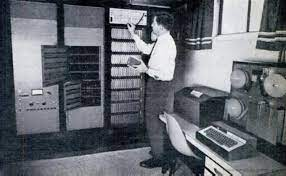
\includegraphics[width=0.65\textwidth]{figures/echo.png}   
\caption{James Sutherland junto al ECHO IV}
\label{fig:echo}
\end{figure}
En la década de 1970, aparecieron los primeros sistemas automáticos de pruebas en edificios públicos y de oficinas de los países más avanzados tecnológicamente por aquel entonces: Alemania, Estados Unidos y Japón. Pero no fue hasta finales de la década siguiente, paralelamente a la evolución de los sistemas informáticos y el desarrollo de los componentes electrónicos, cuando se comenzaron a implementar en domicilios particulares. \\\\
La aparición en 1983 del cableado estructurado facilitó el conexionado de los diversos componentes y redes que componen los sistemas domóticos, lo que propagó su implementación en rascacielos o grandes oficinas comerciales. Esto posibilitó una eficiencia y un ahorro de consumo inédito hasta el momento, propiciando así su auge en el ámbito global. \\\\
Estas instalaciones primitivas comenzaron a programarse informáticamente en Estados Unidos en 1984 mediante el software SAVE. Eran regidas por el protocolo de comunicación X-10 y actuadas por los usuarios por medio de accionadores por control remoto, transmitiendo los datos a través de las líneas de baja tensión. \\\\
De la mano de la popularización de los servicios de tele-asistencia en los años 90 y la revolución que supuso la extensión del uso de internet, la domótica evolucionó hasta los complejos sistemas que podemos encontrar en una vivienda actual común: sistemas en los que se permite un control más amplio y exhaustivo, incluso de manera remota, de numerosos dispositivos tecnológicos vía Wi-Fi, gracias al desarrollo de protocolos de comunicación como ZigBee. \\\\
Actualmente, la domótica se encuentra experimentando un fuerte crecimiento gracias a su precio más accesible, que permite que esta tecnología esté cada día al alcance de más gente. Por una parte, los avances tecnológicos abaratan los costes de instalación y mantenimiento de los componentes mecánicos. Igualmente, se ha facilitado la experiencia del usuario y mejorado la usabilidad del sistema gracias a la aparición de numerosas aplicaciones que nos permiten controlar nuestros hogares desde cualquier lugar del planeta en tiempo real. 


\section{Estado del Arte}
Con muy pocos años de rodaje, la domótica se ha convertido en uno de los sectores con mayor relevancia y perspectiva de incremento y potenciación futura, gracias a los avances tecnológicos recogidos en numerosos artículos y publicaciones, como el caso de “Domótica: Edificios Inteligentes” \cite{EI:2004}. Estos avances que van de la mano de otros sectores como por ejemplo, el social, con su continua lucha hacia la inclusión total de la población o el diseño de interiores y su afán por convertir nuestros hogares en una prolongación más de nuestro cuerpo, para hacernos sentir lo más cómodos y confortables posible. Pero es, sin duda, la apuesta de la sociedad por la inclusión de esta tecnología en el sector de la construcción lo que provoca su gran avance, mejorando e incluso desarrollando nuevas funcionalidades, lenguajes de programación y protocolos de comunicación.\\\\

Esta evolución ha ido permitiendo de manera progresiva que, poco a poco los sistemas domóticos integren una mayor cantidad de mecanismos, ampliando así el catálogo de funcionalidades que pueden ofrecer, a la par que estos son diseñados para actuar de manera más independiente y autónoma. En un principio, los sistemas domóticos eran centralizados, es decir, todos los mecanismos y sus parámetros eran controlados desde una central; en cambio, a día de hoy, los elementos son inteligentes y pueden portar su propia programación, y actuar en consonancia a ella, convirtiéndose en sistemas descentralizados. Esta cualidad, obtenida con el paso del tiempo y la integración de los avances tecnológicos, ha permitido la mejora de 4 áreas fundamentales en el control de una vivienda: la seguridad, la gestión energética, el confort y las comunicaciones  \cite{Andes:2011}, como se demostró en la Universidad Católica del Ecuador \cite{Ecuador:2017}, donde gracias a la mejora de los protocolos de comunicación, en especial, la implementación del X10 \cite{esther:2009}, se pudo domotizar una escuela al completo, mejorando así la calidad de la enseñanza y la satisfacción de sus alumnos y profesores.\\\\
En el caso del ámbito de la seguridad doméstica, la domótica explota de manera mucho más eficiente que los sistemas tradicionales, en al menos 3 de los campos más demandados \cite{iecor}, integrándolos con el resto de dispositivos. Uno de estos campos será el enfocado hacia las alarmas técnicas, que mediante sistemas sensoriales, podrán avisar al usuario de que existe un elemento en la casa que se encuentra averiado o realizando un mal funcionamiento, como pueda ser una tubería de agua rota o un horno demasiado caliente que quema la comida. Si el problema cuenta con una mayor gravedad o se requiere controlar espacios de manera más certera, incluso se podrán conectar estas alarmas con los servicios de emergencia o reparación profesionales, como pueden ser los bomberos. \\\\
Haciendo uso de esa misma capacidad de conectar con sistemas externos, encontramos los otros 2 campos: la seguridad de los bienes, que mediante detectores de presencia y diferentes actuadores, como alarmas sonoras o cegadoras, tratara de evitar la entrada o sustracción de bienes de la vivienda, enviando un aviso al cuerpo de policía; y la teleasistencia, muy útil especialmente para personas mayores o enfermas, que podrán conectar con los servicios sanitarios que requieran con la simple pulsación de un botón.\\\\
En cuanto a la gestión energética, la domótica también se ha hecho un hueco en este sector gracias a la integración de elementos como temporizadores, termostatos, relojes temporizadores con otros más habituales, como los contadores de consumo, que conectados a través de actuadores, crean un sistema eficiente de ahorro de energía.\\\\
Desde el comienzo de su aplicación en los años 80, principalmente en EE.UU. y Japón, y su popularización en los 90 en países de Europa como Francia, Alemania u otros países nórdicos, la domótica ha ido de la mano del mercado de la construcción. Este sector, ya desde 2004, impulsaba el crecimiento del uso de la domótica al ser instalado en el 7\% \cite{Ikei:2004} de las nuevas promociones, propiciando la aparición de comités de expertos que comienzan a regular y afianzar el termino domótica, creando en Europa en 2006 la Especificación de AENOR EA2006 \cite{direct:2004}, pionera de este sector, que determinaría los requisitos mínimos que debía dispensar una vivienda para poder ser considerada domótica. Una vez fijados la base del concepto, instituciones  como el Ministerio de Industria y Turismo pronto comenzaron a realizar otro conjunto de guías y manuales, como por ejemplo, la Guía Técnica de Aplicación ITC-BT-51 \cite{BOE:2002} creada en 2007, que sentaba catedra acerca de “los requisitos específicos de la instalación de los sistemas de automatización, gestión técnica de la energía y seguridad para viviendas y edificios, también conocidos como sistemas domóticos”.\\\\ 
El estallido de la burbuja inmobiliaria acompañado a la crisis financiera global de finales de la primera década del siglo provoco una caída del 62\% en la construcción de nuevas viviendas, truncando la tendencia a la alza que tenía el mercado domótico, llegando a traducir su incidencia en un descenso del 60\% de la instalación en vivienda nueva \cite{AED:2011}, lejos de la previsiones vaticinadas por numerosos medios \cite{mundo:2010} \cite{Info:2008}, que predecía un 25\% de viviendas de nueva obra con instalación domótica integrada en el año 2010.\\\\
 La domótica, actualmente, se encuentra en continuo desarrollo y enfrentándose a diversos conflictos o problemas como su alto coste de instalación, la falta de personal cualificado, la normalización de los diversos softwares que existen en los diferentes mercados del mundo, la dependencia del sistema eléctrico o los problemas del mundo de la informática, como pueden ser los hackers \cite{cerda:2018}, dando sensación de inseguridad dentro de la tu propia casa. Por lo tanto, es una ciencia con un potencial muy grande pero debe superar los problemas básicos con que se encuentra cualquier tecnología durante su fase de desarrollo, para poder crecer y convertirse en un referente en cuanto a los servicios que ofrece y lo óptimo de sus resultados.\\\\
A día de hoy, ya se ha implementado en 44 millones de hogares en Europa y Norte América \cite{HT:2014}, brindando así la certeza del potencial con el que cuenta esta tecnología y el crecimiento exponencial en el que se encuentra: en 2015, en Europa existían únicamente 5.3 millones de viviendas frente a los 18 millones de 2020. Esta cifra lejos de congelarse, continua en crecimiento con la meta de alcanzar un 20\% de casas domotizadas del total en Europa para el año 2025 \cite{Berg:2020}. En cuanto a su desarrollo en España, se espera que el auge de la domótica logre alcanzar un 300\% para el año 2024, realizándose en casi un 60\% de instalaciones de nueva construcción \cite{Portal:2020} y encontrándose ya en el 40\% de los hogares en forma de dispositivo inteligente.

\newpage
\section{¿Qué es KNX?}

Tal y como se menciona en su “biografía” \cite{KNX:2021}, la Asociación KNX fue fundada en 1990 tras la fusión de otras dos asociaciones europeas: BCI, que operaba con el protocolo domótico Batibus  en Francia, pero que en la actualidad ya se encuentra obsoleto; y la European Home Systems Association, que mantuvo los estándares de su sistema EHS a la hora de desarrollar la tecnología KNX.\\\\
Los principales objetivos de esta asociación se fijaron como meta la definición de un nuevo protocolo de programación abierto que fuese consolidado en el mundo entero como estándar. Este protocolo y sus datos son transmitidos vía BUS del tipo \textit{Twisted Pair (TP)} a todos los componentes del sistema, ya que de esta manera se podría descentralizar los componentes, facilitando y reduciendo los trabajos de cableado. Este sistema también permitía que las funciones y llamadas pudiesen ser compartidas por varios de los mecanismos instalados, dando mayor libertad de diseño y, por tanto, añadiendo un valor muy importante a la domótica.\\\\
Este protocolo permite transmitir los datos KNX mediante diferentes vías, en función del área de aplicación que vaya a tener la instalación domótica: el más habitual, es el ya mencionado \textit{Twisted Pair}, que se instalará en viviendas de nueva construcción o en instalaciones en las que se precise una reforma que incluya el recableado intrapared y aportará la mayor capacidad de transmisión. También se puede encontrar la transmisión a través de la red eléctrica, perdiendo fiabilidad de transmisión al no tratarse de una red tan estable pero con la ventaja de no necesitar una instalación de cable adicional, evitando obras y reformas en las casas. Por otro lado, encontramos los medios inalámbricos: mediante radiofrecuencia o vía Ethernet/WIFI, siendo utilizada esta última en grandes instalaciones que precisen de una rapidez mayor en las comunicaciones y utilicen cualquier dispositivo móvil para su control y/o visualización.\\\\
Este protocolo ejecuta envíos de paquetes de datos denominados Telegramas que tendrán la siguiente estructura: 
\begin{figure}[H]
\centering
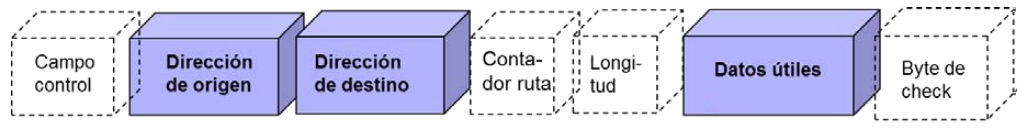
\includegraphics[width=1\textwidth]{figures/telegrama.png} 
\caption{Estructura general de un telegrama}
\label{fig:telegrama}
\end{figure}
En la imagen \ref{fig:telegrama} se ve que su estructura comienza con un campo de control que tendrá como función la de indicar al sistema que es un telegrama real y no cualquier ruido o perturbación que pueda aparecer en la línea. A continuación aparecen las direcciones de origen y de destino, que indicarán que mecanismo deberá recibir la información y de donde proviene esta. También será necesaria la inclusión de un contador de ruta, que irá añadiendo valores a su variable de conteo por cada subsistema que atraviese, evitando así la propagación de información innecesaria entre las diferentes instalaciones que se encuentren interconectadas y la aparición de bucles que puedan llegar a colapsar el BUS. Además de encontrarse la información propiamente útil del telegrama, este contara con un parámetro que indica su longitud, y al final un espacio de memoria para poder informar al sistema de la recepción de los telegrama, evitando así su repetición de envió con el uso de este acuse de recibo. En estos datos útiles, el telegrama indicará al mecanismo la acción o la información que se desea transmitir, como la orden de subir una persiana o el apagado de un punto de luz.\\\\
En el siguiente gráfico \ref{fig:estructura} se muestra la estructura de la topología de máximo tamaño permitida en una instalación KNX. Esta contará con una línea principal o troncal de la que “colgarán” el resto de elementos, ya sea un acoplador de área o directamente los dispositivos mecánicos a instalar, teniendo como capacidad máxima un total de 64 de la suma de ambos.  
\begin{figure}[H]
\centering
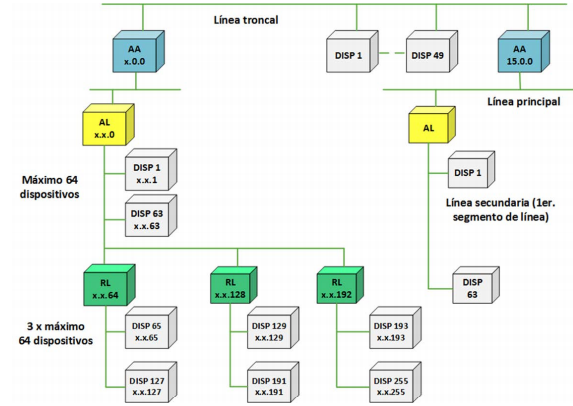
\includegraphics[width=0.95\textwidth]{figures/estructura.png} 
\caption{Estructura máxima de una instalación KNX TP}
\label{fig:estructura}
\end{figure}

En el caso de utilizar un acoplador de área,  permitirá al sistema incluir otros 64 elementos “colgando” de ella, ya sean acopladores de línea o dispositivos. En el caso de que la instalación precise de ampliar el número máximo de elementos “colgantes”, se podrá hacer uso de los repetidores de línea, permitiendo cada implementación una adición extra de otros 64 elementos, hasta un máximo de 255 en total. Para evitar la ya comentada propagación innecesaria de datos entra partes del sistema, tanto los acopladores de línea como los de área contarán con un filtro que evitará este suceso, creando los “telegramas internos de línea o área”. \\\\
Cada uno de estos “pisos” serán los que incrementen en 1 el valor del contador interno de cada telegrama, debiéndose tener en cuenta que el máximo permitido es de 6, por lo que se deberá tener en cuenta este factor a la hora de comunicar dispositivos en instalaciones de gran tamaño. Un ejemplo de comunicación vía telegrama no permitido sería el representado en la Imagen \ref{fig:contador}, donde un dispositivo que cuelga de un acoplador de área, seguido de un acoplador de línea en un repetidor de línea, trata de comunicarse con otro dispositivo que se encuentra en las mismas condiciones topológicas. Como se puede observar el contador (CR) va bajando su valor a medida que pasa por ellos, alcanzando su valor minimo (0) antes de llegar al dispositivo receptor.
\begin{figure}[H]
\centering
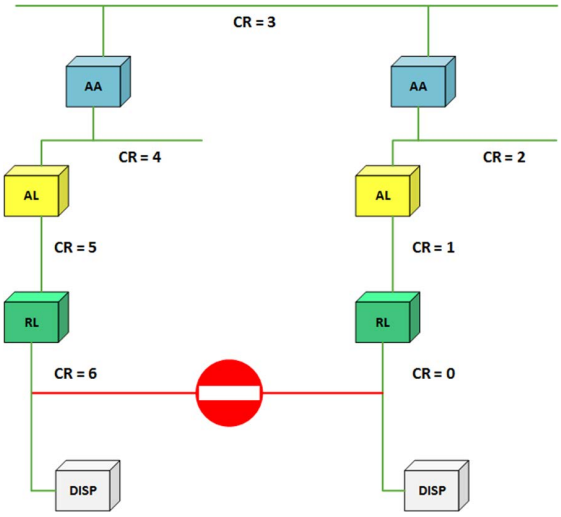
\includegraphics[width=0.65\textwidth]{figures/contador.png} 
\caption{Ejemplo de contador de etapas de un telegrama}
\label{fig:contador}
\end{figure}
